\documentclass{article}


\usepackage{array}
\usepackage{amsfonts}
\usepackage{amsmath}
\usepackage{geometry}
\usepackage{stmaryrd}
\usepackage{xcolor}
\usepackage{graphicx}
\usepackage{appendix}
\title{IEOR 240 : Homework 5}
\author{Arnaud Minondo}
\begin{document}
\maketitle
\section*{Dorian Auto}
Let $x_1,x_2,x_3$ be the respective amount of Compact, MidSize, Large cars.\\Let $\forall i \in\{1,2,3\}, b_i = \left\{\begin{array}{cc}
    1 & \text{if } x_i>0\\
    0 & \text{otherwise}\\
\end{array}\right.$.\\
The optimization problem corresponding to Dorian Auto case is :
\begin{equation}
    \boxed{
        \begin{split}
            &\max(2000x_1+3000x_2+4000x_3) \\
            &\begin{split}
                \text{ s.t. } & 30x_1+25x_2+40x_3\leq 60 000\\
                &1.5x_1+3x_2+5x_3 \leq 6000\\
                &1000b_1\leq x_1\leq 4000b_1 \\
                &1000b_2\leq x_2\leq 4000b_2\\
                &1000b_3\leq x_3\leq 4000b_3\\
                &x_1,x_2,x_3\ge 0\\
            \end{split}\\
        \end{split}}
\end{equation}\\\\
\section*{Coach Night}
Let $T = (t_1,t_2,t_3,t_4,t_5,t_6,t_7)$ be the lineup starting. $\forall i \in \{1,2,3,4,5,6,7\}, t_i$ is binary, 1 if the player $i$ starts, 0 otherwise.
The problem is : 
\begin{equation}
    \boxed{
    \begin{split}
    &\max(3t_1+2t_2+2t_3+3t_4+3t_5+3t_6+t_7) \\
    & \begin{split}
        \text{s.t. } & t_1+t_3+t_5+t_7 \ge 4\\
        &t_3+t_4+t_5+t_6+t_7 \ge2\\
        &t_2+t_4+t_6 \ge 1\\
        &\frac{1}{5}(3t_1+2t_2+2t_3+t_4+3t_5+3t_6+3t_7)\ge 2\\
        &\frac{1}{5}(3t_1+1t_2+3t_3+3t_4+3t_5+1t_6+2t_7)\ge 2\\
        &\frac{1}{5}(1t_1+3t_2+2t_3+3t_4+3t_5+2t_6+2t_7)\ge 2\\
        &\frac{1}{5}(3t_1+2t_2+2t_3+3t_4+3t_5+3t_6+t_7)\ge 2\\
        &t_6\leq1-t_3\\
        &\frac{1}{2}(t_4+t_5)\ge t_1\\
        &t_2+t_3 \ge 1\\
        &t_1+t_2+t_3+t_4+t_5+t_6+t_7=5\\
    \end{split}\\
    \end{split}}
\end{equation}\\\\
I assumed that the condition : ``Either player 2 or player 3 must start'' is equivalent to at least one them has to start.
\section*{Investment Management Company}
Let $p_1,p_2,p_3,p_4,p_5,p_6$ be the binary corresponding to $p_i = 1$ if project $i$ is chosen 0 otherwise. 
\begin{equation}
    \boxed{
    \begin{split}
    &\max(0.1222p_1+0.1536p_2+0.1128p_3+0.171p_4+0.114p_5+0.2304p_6)  \\
    &\begin{split}
    \text{s.t. } & 1.3p_1+0.8p_2+0.6p_3+1.8p_4+1.2p_5+2.4p_6\leq 4\\
    & \frac{1}{p_1+p_2+p_3+p_4+p_5+p_6}(6p_1+4p_2+6p_3+5p_4+5p_5+4p_6) \leq 5\\
    & p_2\ge p_1\\
    & p_5\ge p_3+p_4-1\\
    \end{split}\\
    \end{split}}
\end{equation}\\\\
\section*{MBA Student, Li Hua}
Let $ = (c_O,c_A,c_{IT},c_F,c_M,c_{OB},c_{P},c_C)$ be the binary variable representing the course chosen by the student.
The problem is :
\begin{equation}
    \boxed{
    \begin{split}
        &\max(0.10c_O+0.04c_A+0.06c_{IT}+0.12c_F+0.08c_M+0.03c_{OB}+0.04c_P+0.05c_C)\\
        &\begin{split}
            \text{s.t. }& 9c_O+7c_A+5C_{IT}+8c_F+5c_M+3c_{OB}+7c_P+10c_C\leq 40\\
        \end{split}\\
    \end{split}}
\end{equation}
In the problem satement it is said that the student has to study 40 hours but if we can have better with less it might be better to reconsider the planning. That's why I put less or equal to rather than equal to 40(Anyway it does not change the optimal solution but it could have).
My result for this problem solved using AMPL is : $C = (1,0,1,1,1,1,0,1)$
\\\\
You can find the code in the appendix. 
\newpage
\begin{appendices}
    \section{.mod file}
    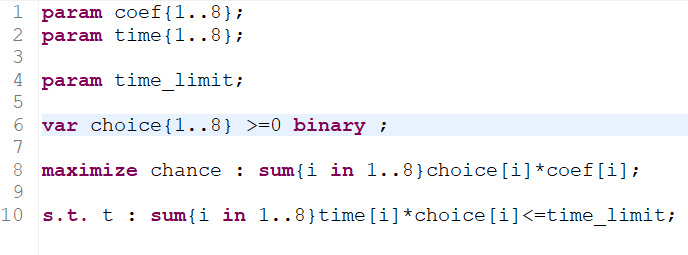
\includegraphics[]{img/mba_mod.png}
    \section{.dat file}
    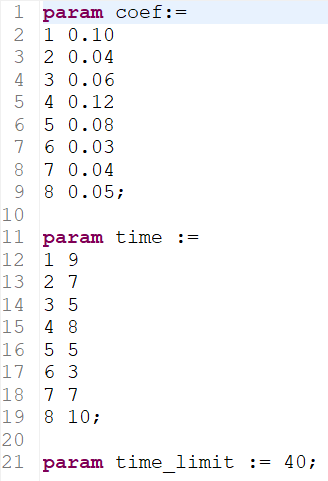
\includegraphics[]{img/mba_dat.png}
    \section{.run file}
    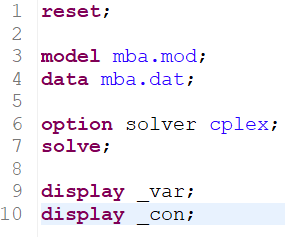
\includegraphics[]{img/mba_run.png}
\end{appendices}

\end{document}